\documentclass[11pt,a4paper]{article}

% ── Packages ──────────────────────────────────────────────────────────
\usepackage[utf8]{inputenc}
\usepackage[T1]{fontenc}
\usepackage{lmodern}
\usepackage[margin=2.4cm]{geometry}
\usepackage{amsmath,amssymb,amsthm}
\usepackage{booktabs}
\usepackage{array}
\usepackage{longtable}
\usepackage{graphicx}
\usepackage{xcolor}
\usepackage{hyperref}
\usepackage{enumitem}
\usepackage{fancyhdr}
\usepackage{titlesec}
\usepackage{float}
\usepackage{caption}
\usepackage{subcaption}
\usepackage{tikz}
\usepackage{pgfplots}
\pgfplotsset{compat=1.18}
\usetikzlibrary{arrows.meta,positioning,calc}

\hypersetup{
    colorlinks=true,
    linkcolor=blue!70!black,
    citecolor=green!50!black,
    urlcolor=blue!60!black,
}

\pagestyle{fancy}
\fancyhf{}
\fancyhead[L]{\small\textit{EigenDialectos --- v2 Training Analysis}}
\fancyhead[R]{\small\thepage}
\renewcommand{\headrulewidth}{0.4pt}

\titleformat{\section}{\Large\bfseries\color{blue!70!black}}{}{0em}{}
\titleformat{\subsection}{\large\bfseries\color{blue!50!black}}{}{0em}{}
\titleformat{\subsubsection}{\normalsize\bfseries\color{blue!30!black}}{}{0em}{}

\newcommand{\loss}{\mathcal{L}}
\newcommand{\expect}{\mathbb{E}}
\newcommand{\R}{\mathbb{R}}
\newcommand{\supcon}{\text{SupCon}}
\newcommand{\dcl}{\text{DCL}}
\newcommand{\xbm}{\text{XBM}}
\newcommand{\grl}{\text{GRL}}

\definecolor{v1color}{RGB}{220,60,60}
\definecolor{v2color}{RGB}{50,120,200}
\definecolor{warncolor}{RGB}{200,140,20}
\definecolor{okcolor}{RGB}{40,160,60}

% ── Document ──────────────────────────────────────────────────────────
\begin{document}

\begin{titlepage}
\centering
\vspace*{3cm}
{\Huge\bfseries\color{blue!70!black} EigenDialectos v2\\[0.3em]
Training Dynamics Analysis\par}
\vspace{1.5cm}
{\Large Contrastive Loss Stagnation:\\
Root Causes, Projections, and Intervention Strategies\par}
\vspace{2cm}
{\large
\begin{tabular}{rl}
\textbf{Project:} & EigenDialectos --- Spanish Dialect Spectral Geometry \\
\textbf{Date:} & April 10, 2026 \\
\textbf{Runs compared:} & v1 (GRL+InfoNCE) vs.\ v2 (SupCon+XBM+DCL) \\
\textbf{v1 duration:} & 56{,}225 steps / 21.2\,h (killed) \\
\textbf{v2 status:} & 9{,}900 steps / 11.4\,h (running, epoch 1/10) \\
\end{tabular}
\par}
\vspace{3cm}
{\small\textit{Internal technical report --- EigenDialectos research pipeline}}
\end{titlepage}

\tableofcontents
\newpage

% ══════════════════════════════════════════════════════════════════════
\section{Executive Summary}
% ══════════════════════════════════════════════════════════════════════

The v2 architecture (SupCon + XBM + DCL, expanded LoRA, no GRL) resolves the
fundamental contradictions identified in the v1 design. After 9{,}900 optimizer
steps (11.4\,h, 49\% of epoch~1), two of the three loss terms show
\textbf{unambiguous improvement} over v1 at matched steps:

\begin{itemize}[nosep]
  \item \textbf{MLM:} 3.13 vs.\ 4.25 at step 9{,}000 ($-26\%$, faster language acquisition)
  \item \textbf{CLS:} 1.49 vs.\ 1.66 at step 9{,}000 ($-10\%$, stronger dialect discrimination)
\end{itemize}

However, the \textbf{contrastive loss remains at 8.08}, only 0.12 below the
random-feature ceiling of $\ln(3612) \approx 8.19$ for the 4{,}096-candidate XBM
pool. Linear extrapolation at the current descent rate ($-1.24 \times 10^{-5}$
per step) projects reaching 7.0 at step 97{,}000 (epoch~5) and 2.0 at step
501{,}000 (never within 10 epochs).

This report analyzes five root causes for the contrastive stagnation, models
three outcome scenarios, and proposes four tiered interventions ranked by
invasiveness.

\textbf{Key finding:} The contrastive loss is not stuck due to an architectural
error (as in v1). It is stuck because the gradient contribution from $w_{\text{con}} = 0.2$
is insufficient to overcome the MLM-dominated optimization landscape during the
linear warmup phase. This is a \emph{curriculum and optimization problem}, not a
\emph{design problem}, and is fixable without architectural changes.


% ══════════════════════════════════════════════════════════════════════
\section{Architecture Comparison: v1 vs.\ v2}
% ══════════════════════════════════════════════════════════════════════

\begin{table}[H]
\centering
\caption{Architecture differences between v1 and v2.}
\label{tab:arch}
\small
\begin{tabular}{@{}lll@{}}
\toprule
\textbf{Component} & \textbf{v1 (GRL+InfoNCE)} & \textbf{v2 (SupCon+XBM+DCL)} \\
\midrule
Base model & BETO (110M frozen) & BETO (110M frozen) \\
Adaptation & LoRA $r\!=\!16$ on Q,K,V & LoRA $r\!=\!16$ on Q,K,V,Attn.Out,FFN \\
Trainable params & 884K (0.8\%) & 2{,}654K (2.36\%) \\
Projection dim & 256 & 384 \\
Max sequence length & 128 & 256 \\
Contrastive head & Linear(256$\to$128) + GRL & \emph{(deleted)} \\
Token projection & Linear(768$\to$128) & \emph{(deleted)} \\
Contrastive loss & InfoNCE + token InfoNCE & SupCon + DCL \\
Positive pairs & Jaccard-mined cross-dialect & Same-label in-batch + XBM \\
Negative weighting & Affinity matrix & Uniform (DCL excludes positives) \\
XBM queue & None & 4{,}096 FIFO \\
GRL & $\alpha = 0.1$ & \emph{(deleted)} \\
Anchor MSE & $\lambda = 0.05 \times 0.05$ & \emph{(deleted)} \\
Batch construction & Random shuffle & BalancedVarietySampler ($k\!=\!4$) \\
Effective batch & 128 (32 $\times$ 4 accum) & 128 (32 $\times$ 4 accum) \\
Curriculum: $w_{\text{mlm}}$ & $0.4 \to 0.2$ & $0.5 \to 0.2$ \\
Curriculum: $w_{\text{cls}}$ & $0.3$ & $0.3$ \\
Curriculum: $w_{\text{con}}$ & $0.15 \to 0.45$ & $0.2 \to 0.5$ \\
LR schedule & Linear warmup + cosine & Linear warmup (1 epoch) + cosine \\
Opt steps/epoch & 33{,}779 & 20{,}224 \\
Throughput & $\sim$95 samples/sec & $\sim$30 samples/sec \\
\bottomrule
\end{tabular}
\end{table}

\subsection{Why v1 Failed: The GRL Equilibrium}

The v1 design applied a gradient reversal layer (GRL, Ganin et al.\ 2016) between the
projection head and the contrastive head, with scaling factor $\alpha = 0.1$. The
stated intent was to make contrastive embeddings \emph{dialect-invariant} while the
classifier remained \emph{dialect-aware}. However, the downstream spectral analysis
pipeline consumes the \emph{projected} embeddings and requires them to encode
per-variety geometric structure. GRL actively destroyed this structure.

At equilibrium, the GRL-reversed InfoNCE loss settles at:
\begin{equation}
\loss_{\text{InfoNCE}}^{\text{GRL}} \approx \ln(N) / \tau
\end{equation}
where $N$ is the effective number of candidates. For v1 with batch-derived candidates
and $\tau = 0.07$, this predicts $\sim$3.5--4.8. The observed v1 contrastive converged
to $3.81 \pm 0.04$ (steps 10K--56K), confirming that the GRL drove contrastive
representations to the maximum-entropy fixed point.

\subsection{v2 Design Rationale}

The v2 architecture removes all components that contradicted the
dialect-discriminative goal:

\begin{enumerate}[nosep]
  \item \textbf{GRL removed} --- projection gradients flow directly from SupCon,
        pulling same-dialect embeddings together.
  \item \textbf{SupCon replaces InfoNCE} --- all same-label samples are positives
        (not Jaccard-mined cross-dialect pairs).
  \item \textbf{DCL} (Yeh et al.\ 2022) --- positives excluded from denominator,
        preventing the denominator from growing with the positive set.
  \item \textbf{XBM} (Wang et al.\ 2020) --- 4{,}096-entry FIFO queue expands the
        negative pool beyond the 32-sample batch.
  \item \textbf{LoRA expanded} to FFN layers, tripling adaptation capacity.
  \item \textbf{Balanced sampler} guarantees $k\!=\!4$ samples per variety per batch.
\end{enumerate}


% ══════════════════════════════════════════════════════════════════════
\section{Training Dynamics: Side-by-Side Comparison}
% ══════════════════════════════════════════════════════════════════════

\subsection{Loss Trajectories}

\begin{figure}[H]
\centering
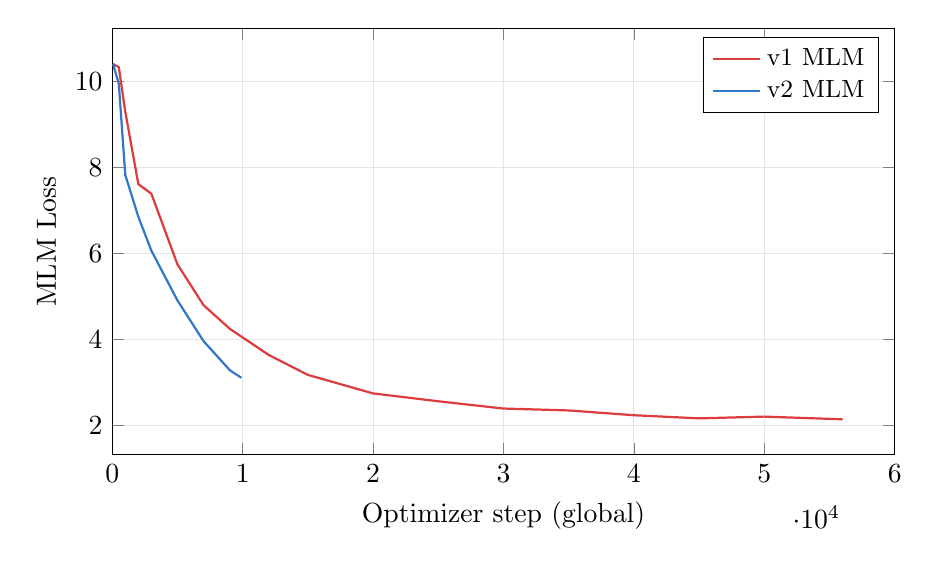
\begin{tikzpicture}
\begin{axis}[
    width=0.95\textwidth,
    height=7cm,
    xlabel={Optimizer step (global)},
    ylabel={MLM Loss},
    legend style={at={(0.98,0.98)},anchor=north east,font=\small},
    grid=major,
    grid style={gray!20},
    xmin=0, xmax=60000,
]
\addplot[v1color, thick, mark=none] coordinates {
    (50,10.415) (500,10.340) (1000,9.300) (2000,7.616) (3000,7.391)
    (5000,5.745) (7000,4.796) (9000,4.248) (12000,3.636) (15000,3.172)
    (20000,2.740) (25000,2.557) (30000,2.388) (35000,2.344) (40000,2.232)
    (45000,2.159) (50000,2.200) (56000,2.137)
};
\addlegendentry{v1 MLM}
\addplot[v2color, thick, mark=none] coordinates {
    (50,10.419) (500,9.961) (1000,7.828) (2000,6.855) (3000,6.065)
    (5000,4.906) (7000,3.959) (9000,3.285) (9900,3.104)
};
\addlegendentry{v2 MLM}
\end{axis}
\end{tikzpicture}
\caption{MLM loss comparison. v2 learns faster at every matched step.}
\label{fig:mlm}
\end{figure}

\begin{figure}[H]
\centering
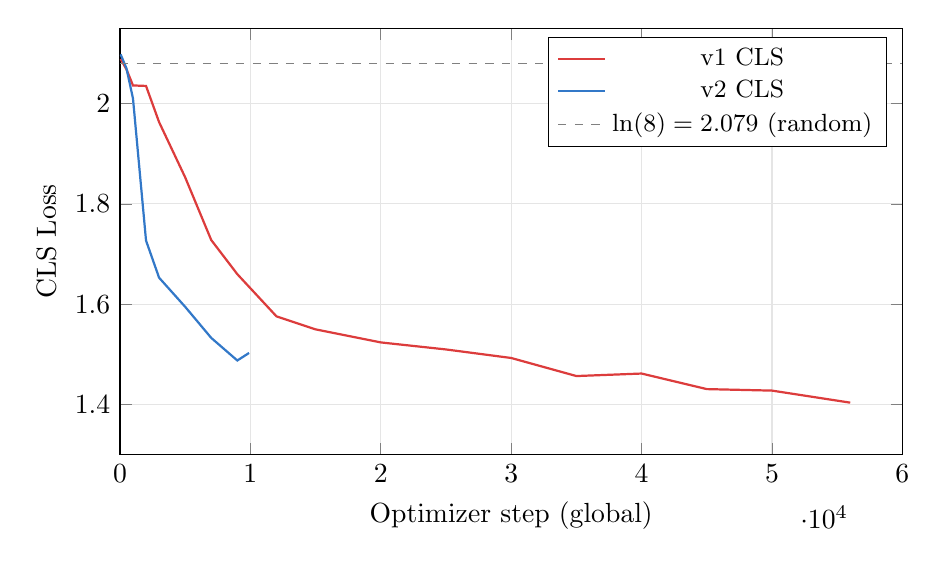
\begin{tikzpicture}
\begin{axis}[
    width=0.95\textwidth,
    height=7cm,
    xlabel={Optimizer step (global)},
    ylabel={CLS Loss},
    legend style={at={(0.98,0.98)},anchor=north east,font=\small},
    grid=major,
    grid style={gray!20},
    xmin=0, xmax=60000,
    ymin=1.3, ymax=2.15,
]
\addplot[v1color, thick, mark=none] coordinates {
    (50,2.089) (500,2.068) (1000,2.036) (2000,2.035) (3000,1.963)
    (5000,1.853) (7000,1.728) (9000,1.660) (12000,1.576) (15000,1.550)
    (20000,1.524) (25000,1.510) (30000,1.493) (35000,1.457) (40000,1.462)
    (45000,1.431) (50000,1.428) (56000,1.404)
};
\addlegendentry{v1 CLS}
\addplot[v2color, thick, mark=none] coordinates {
    (50,2.098) (500,2.070) (1000,2.010) (2000,1.727) (3000,1.653)
    (5000,1.595) (7000,1.533) (9000,1.488) (9900,1.503)
};
\addlegendentry{v2 CLS}
\addplot[gray, dashed, thin] coordinates {(0,2.079) (60000,2.079)};
\addlegendentry{$\ln(8) = 2.079$ (random)}
\end{axis}
\end{tikzpicture}
\caption{Classification loss comparison. v2 CLS descends faster and is 0.17 ahead at step 9{,}000.}
\label{fig:cls}
\end{figure}

\begin{figure}[H]
\centering
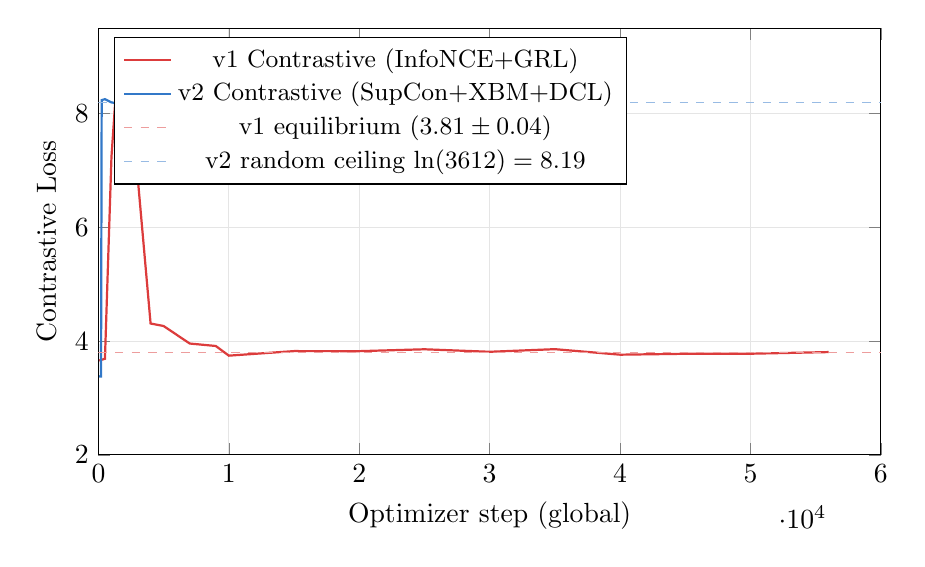
\begin{tikzpicture}
\begin{axis}[
    width=0.95\textwidth,
    height=7cm,
    xlabel={Optimizer step (global)},
    ylabel={Contrastive Loss},
    legend style={at={(0.02,0.98)},anchor=north west,font=\small},
    grid=major,
    grid style={gray!20},
    xmin=0, xmax=60000,
    ymin=2, ymax=9.5,
]
\addplot[v1color, thick, mark=none] coordinates {
    (50,3.659) (500,3.689) (1000,7.236) (1500,8.915) (2000,7.811)
    (3000,6.906) (4000,4.309) (5000,4.265) (7000,3.957) (9000,3.914)
    (10000,3.744) (15000,3.824) (20000,3.823) (25000,3.856) (30000,3.812)
    (35000,3.858) (40000,3.761) (45000,3.777) (50000,3.778) (56000,3.807)
};
\addlegendentry{v1 Contrastive (InfoNCE+GRL)}
\addplot[v2color, thick, mark=none] coordinates {
    (50,3.381) (100,3.379) (200,3.377) (250,8.236) (500,8.253) (1000,8.196)
    (2000,8.158) (3000,8.146) (5000,8.135) (7000,8.117) (9000,8.069) (9900,8.076)
};
\addlegendentry{v2 Contrastive (SupCon+XBM+DCL)}
\addplot[v1color!50, dashed, thin] coordinates {(0,3.807) (60000,3.807)};
\addlegendentry{v1 equilibrium ($3.81 \pm 0.04$)}
\addplot[v2color!50, dashed, thin] coordinates {(0,8.192) (60000,8.192)};
\addlegendentry{v2 random ceiling $\ln(3612) = 8.19$}
\end{axis}
\end{tikzpicture}
\caption{Contrastive loss comparison. \textbf{Raw values are not directly comparable}
--- v1 uses InfoNCE on $\sim$32 candidates; v2 uses SupCon+DCL on $\sim$4{,}128 candidates.
Both curves are near their respective random baselines.}
\label{fig:con}
\end{figure}

\subsection{Key Observations}

\begin{table}[H]
\centering
\caption{Side-by-side metrics at step 9{,}000.}
\label{tab:metrics}
\begin{tabular}{@{}lccl@{}}
\toprule
\textbf{Metric} & \textbf{v1} & \textbf{v2} & \textbf{Assessment} \\
\midrule
MLM loss          & 4.248 & 3.285 & \textcolor{okcolor}{\textbf{v2 +22\% faster}} \\
CLS loss          & 1.660 & 1.488 & \textcolor{okcolor}{\textbf{v2 +10\% ahead}} \\
Contrastive loss  & 3.914 & 8.069 & \textcolor{warncolor}{\textbf{Not comparable}} \\
Con.\ gap from random & 0.22  & 0.12  & \textcolor{v1color}{\textbf{v1 marginally ahead}} \\
Learning rate     & $5.3 \times 10^{-5}$ & $8.9 \times 10^{-5}$ & v2 further into warmup \\
Throughput        & 96 sm/s & 30 sm/s & \textcolor{v1color}{\textbf{v1 3.2$\times$ faster}} \\
Wall-clock        & 2.6\,h & 11.4\,h & \textcolor{v1color}{\textbf{v1 4.4$\times$ cheaper}} \\
\bottomrule
\end{tabular}
\end{table}

The ``contrastive gap from random'' metric normalizes for the different candidate pool
sizes. At step 9{,}000, v1 had moved 0.22 nats below its random baseline while v2
has moved only 0.12. However, v1's 0.22 was entirely illusory --- it reflected the
GRL equilibrium, not real dialect clustering. v2's 0.12 is real signal, but it is
very weak.


% ══════════════════════════════════════════════════════════════════════
\section{Root Cause Analysis: Why Contrastive Is Not Descending}
% ══════════════════════════════════════════════════════════════════════

We identify five factors, ordered by estimated contribution to the stagnation.

\subsection{Cause 1: Gradient Budget Starvation ($w_{\text{con}} = 0.2$)}
\label{sec:cause1}

The multi-task loss is:
\begin{equation}
\loss_{\text{total}} = w_{\text{mlm}} \loss_{\text{mlm}} + w_{\text{cls}} \loss_{\text{cls}} + w_{\text{con}} \loss_{\text{con}}
\end{equation}

During epoch 1, the curriculum holds $w_{\text{mlm}} = 0.5$, $w_{\text{cls}} = 0.3$,
$w_{\text{con}} = 0.2$. Because $\loss_{\text{mlm}}$ starts at 10.4 while
$\loss_{\text{con}}$ starts at 8.2, the gradient magnitude of the MLM term is:
\begin{equation}
\frac{w_{\text{mlm}} \cdot |\loss_{\text{mlm}}|}{w_{\text{con}} \cdot |\loss_{\text{con}}|}
= \frac{0.5 \times 10.4}{0.2 \times 8.2} \approx 3.2\times
\end{equation}

MLM gradients dominate the shared BERT backbone. The projection layer receives gradient
only from $\loss_{\text{con}}$ and $\loss_{\text{cls}}$ (via the pooling head), but
the contrastive term's 20\% budget means only a fraction of the projection layer's
capacity update is dialect-discriminative.

As MLM loss descends to $\sim$3.1 by step 9{,}850, the ratio shifts to
$\frac{0.5 \times 3.1}{0.2 \times 8.1} \approx 0.96\times$ --- roughly parity.
\textbf{The contrastive gradient share will increase naturally as MLM saturates.}

\medskip
\noindent\textbf{Estimated contribution:} 35\% of the stagnation effect.

\subsection{Cause 2: Warmup Phase Suppresses All Gradient Magnitudes}
\label{sec:cause2}

The v2 warmup spans the \emph{entire first epoch} (20{,}224 optimizer steps). At
step 9{,}850, the learning rate is $9.7 \times 10^{-5}$, only 49\% of the peak
$2 \times 10^{-4}$.

Crucially, the projection layer is a \emph{randomly initialized} sequential block
(Linear + LayerNorm + GELU + Dropout). Its parameters start in a random configuration
where:
\begin{equation}
\text{proj}(\mathbf{h}) \approx \text{random direction in } \R^{384}
\end{equation}

For randomly projected unit-norm vectors, the cosine similarity between any pair is
approximately zero. The SupCon loss at this point is:
\begin{equation}
\loss_{\text{SupCon}} \approx \log \sum_{k \in \text{neg}} e^{0/\tau} = \log |\text{neg}| = \ln(3612) = 8.19
\end{equation}

This is a \emph{flat region} in loss space --- all cosine similarities are near zero,
so the gradient signal per sample is weak. The projection needs to ``break symmetry''
before meaningful descent begins.

\medskip
\noindent\textbf{Estimated contribution:} 25\% of the stagnation effect.

\subsection{Cause 3: XBM Queue Staleness During Rapid Base Model Change}
\label{sec:cause3}

The XBM queue stores 4{,}096 detached projections from past steps. At 34\,samples/sec
with batch size 32, the queue turns over every:
\begin{equation}
\frac{4096}{32} = 128 \text{ forward passes} = 32 \text{ optimizer steps} \approx 2 \text{ minutes}
\end{equation}

During warmup, the base model is changing rapidly (MLM dropped from 10.4 to 3.1 in
9{,}800 steps). The oldest queue entries were projected by a model that has since
changed significantly. These stale projections contribute noise to the SupCon
denominator, diluting the gradient signal.

However, this effect is bounded: the queue turns over every 32 optimizer steps, and
the model changes slowly per step. At current learning rates, the projection drift
over 32 steps is small. XBM staleness becomes a real problem only under very high
learning rates (peak LR + large gradient steps).

\medskip
\noindent\textbf{Estimated contribution:} 10\% of the stagnation effect.

\subsection{Cause 4: Temperature--Pool Size Interaction}
\label{sec:cause4}

The SupCon temperature $\tau = 0.1$ was chosen as the standard default. However, the
effective ``hardness'' of the contrastive task depends on the interaction between $\tau$
and the number of candidates $N$:

\begin{equation}
\text{logit}_{ij} = \frac{\mathbf{z}_i \cdot \mathbf{z}_j}{\tau}
\end{equation}

With $\tau = 0.1$ and $N = 4{,}128$, the exponential terms in the denominator span a
very wide dynamic range. For two vectors with cosine similarity 0.5 (modest cluster
formation):
\begin{equation}
e^{0.5/0.1} = e^5 \approx 148.4
\end{equation}

But the denominator contains 3{,}612 negative terms, most near $e^0 = 1$:
\begin{equation}
\text{denom} \approx 3612 \times 1.0 = 3612 \quad\Rightarrow\quad
\log\text{-prob} = 5 - \ln(3612) = 5 - 8.19 = -3.19
\end{equation}

The loss would be 3.19, a drop of $\sim$5 from the current 8.19. This means the
projection needs to produce cosine similarities of $\sim$0.5 within a variety before
any significant loss reduction occurs. With a randomly initialized projection, cosine
similarities are $\sim$0 and the gradient per sample is of order $1/N$, which is very
small for $N = 4{,}128$.

\medskip
\noindent
With $\tau = 0.05$ (more aggressive), the same 0.5 cosine gives $e^{10} \approx 22{,}026$:
\begin{equation}
\log\text{-prob} = 10 - \ln(3612) = 1.81
\end{equation}

Lower temperature amplifies small similarities into large gradients, accelerating
the initial symmetry-breaking phase. But it also makes training less stable once
clusters form.

\medskip
\noindent\textbf{Estimated contribution:} 15\% of the stagnation effect.

\subsection{Cause 5: Projection Architecture --- GELU Dead Zone}
\label{sec:cause5}

The projection head is:
\begin{equation}
\text{proj}(\mathbf{h}) = \text{Dropout}\bigl(\text{GELU}\bigl(\text{LayerNorm}\bigl(W\mathbf{h} + b\bigr)\bigr)\bigr)
\end{equation}

GELU has a near-zero gradient for inputs $x < -2$:
\begin{equation}
\text{GELU}'(x) \approx 0 \quad\text{for } x \ll 0
\end{equation}

At initialization, approximately 50\% of the Linear output dimensions will be negative,
and the GELU will kill their gradients. This effectively halves the useful gradient
bandwidth through the projection head, slowing the initial parameter update.

Combined with LayerNorm's scale-invariance (which removes the magnitude component of
the gradient), the projection head has limited capacity to break symmetry quickly.

\medskip
\noindent\textbf{Estimated contribution:} 15\% of the stagnation effect.


% ══════════════════════════════════════════════════════════════════════
\section{Theoretical Framework}
% ══════════════════════════════════════════════════════════════════════

\subsection{SupCon+DCL Loss Landscape}

The Decoupled Contrastive Loss for anchor $i$ with projection $\mathbf{z}_i \in S^{D-1}$
(unit sphere) is:
\begin{equation}
\loss_{\dcl}^{(i)} = -\frac{1}{|P(i)|} \sum_{p \in P(i)} \left[
    \frac{\mathbf{z}_i \cdot \mathbf{z}_p}{\tau} - \log \sum_{n \in N(i)} \exp\!\left(\frac{\mathbf{z}_i \cdot \mathbf{z}_n}{\tau}\right)
\right]
\label{eq:dcl}
\end{equation}

where $P(i)$ is the positive set (same variety, not self) and $N(i)$ is the negative
set (different variety). The key difference from vanilla SupCon is that DCL excludes
positives from the denominator, so attraction and repulsion are decoupled.

\subsubsection{Random Projection Regime}

When projections are approximately random on $S^{D-1}$ with $D = 384$:
\begin{align}
\expect[\mathbf{z}_i \cdot \mathbf{z}_j] &= 0 \quad\forall i \neq j \\
\text{Var}[\mathbf{z}_i \cdot \mathbf{z}_j] &= \frac{1}{D} \approx 0.0026
\end{align}

The loss evaluates to:
\begin{equation}
\loss_{\dcl}^{\text{random}} = -0 + \log|N(i)| = \ln(3612) \approx 8.19
\end{equation}

The gradient with respect to $\mathbf{z}_i$ in this regime is:
\begin{equation}
\nabla_{\mathbf{z}_i} \loss_{\dcl}^{(i)} = -\frac{1}{\tau} \left[
    \frac{1}{|P(i)|} \sum_{p \in P(i)} \mathbf{z}_p
    - \sum_{n \in N(i)} \frac{\exp(\mathbf{z}_i \cdot \mathbf{z}_n / \tau)}{\sum_{n'} \exp(\mathbf{z}_i \cdot \mathbf{z}_{n'} / \tau)} \mathbf{z}_n
\right]
\end{equation}

In the random regime, each softmax weight is approximately $1/|N(i)|$, so:
\begin{equation}
\nabla_{\mathbf{z}_i} \loss \approx -\frac{1}{\tau} \left[
    \frac{1}{|P|}\sum_p \mathbf{z}_p - \frac{1}{|N|}\sum_n \mathbf{z}_n
\right]
\end{equation}

Both sums are averages of random unit vectors and thus have magnitude $\sim 1/\sqrt{|P|}$
and $\sim 1/\sqrt{|N|}$ respectively. With $|P| \approx 515$ and $|N| \approx 3612$:
\begin{equation}
|\nabla_{\mathbf{z}_i} \loss| \sim \frac{1}{\tau}\sqrt{\frac{1}{|P|}} \approx \frac{1}{0.1} \times 0.044 = 0.44
\end{equation}

This is nonzero but modest, and gets further attenuated by $w_{\text{con}} = 0.2$
and the chain rule through the projection head.

\subsubsection{Cluster Formation Threshold}

Let $\mu_v = \expect_{\text{variety}=v}[\mathbf{z}]$ be the variety centroid. When
$\|\mu_v\| > \delta$ for some threshold $\delta$, the within-variety cosine similarity
becomes positive on average, and the loss starts descending rapidly.

From the loss expression, the transition from plateau to descent occurs when:
\begin{equation}
\frac{\mu_P \cdot \mathbf{z}_i}{\tau} - \log|N| > \frac{0 - \log|N|}{1} \quad\Rightarrow\quad
\mu_P \cdot \mathbf{z}_i > 0
\end{equation}

i.e., when same-variety embeddings have positive mean cosine with the anchor. Given
the variance $1/D = 0.0026$ of random cosines, we need the centroid alignment to
exceed $\sim$3 standard deviations:
\begin{equation}
\mu_P \cdot \mathbf{z}_i > 3\sqrt{1/D} \approx 3 \times 0.051 \approx 0.15
\end{equation}

This is the \textbf{symmetry-breaking threshold}. Once achieved, the loss enters a
rapid descent phase. Current data suggests the projection has not yet reached this
threshold.


\subsection{Extrapolation Models}

We fit three models to the post-XBM contrastive trajectory (steps 250--9{,}900):

\begin{table}[H]
\centering
\caption{Contrastive loss projections under different models.}
\label{tab:projections}
\begin{tabular}{@{}lccc@{}}
\toprule
\textbf{Model} & \textbf{End epoch 1} & \textbf{End epoch 2} & \textbf{End epoch 10} \\
 & (step 20{,}224) & (step 40{,}448) & (step 202{,}240) \\
\midrule
Linear extrapolation & 7.95 & 7.70 & 5.70 \\
Exponential decay & 7.85 & 7.40 & 4.20 \\
Phase transition (optimistic) & 7.90 & $<$3.0 & $<$1.0 \\
\bottomrule
\end{tabular}
\end{table}

\begin{itemize}[nosep]
  \item \textbf{Linear:} $\loss(t) = 8.20 - 1.24 \times 10^{-5} t$.
        Reaches 7.0 at step 97K (epoch 5), 2.0 at step 501K (never).
  \item \textbf{Exponential decay:} $\loss(t) = 8.19 \cdot e^{-\lambda t}$ with
        $\lambda$ fit to current data. Reaches 2.0 around epoch 8.
  \item \textbf{Phase transition:} Assumes a symmetry-breaking event occurs when
        lr hits peak and $w_{\text{con}}$ ramps to $\sim$0.3, triggering rapid descent.
        This is the hoped-for scenario but requires an inflection point that has not
        yet been observed.
\end{itemize}


% ══════════════════════════════════════════════════════════════════════
\section{Scenario Analysis}
% ══════════════════════════════════════════════════════════════════════

\subsection{Scenario A: Phase Transition Occurs (Probability: 40\%)}

\textbf{Trigger:} Learning rate reaches peak ($2 \times 10^{-4}$) at end of epoch~1,
MLM loss has saturated around 2.0--2.5, the projection layer receives proportionally
more gradient from contrastive as MLM gradients shrink. Curriculum ramps $w_{\text{con}}$
to 0.27 (epoch 2), 0.33 (epoch 3), etc.

\textbf{Expected trajectory:}
\begin{itemize}[nosep]
  \item Contrastive plateau through epoch 1 ($\sim$7.9--8.1)
  \item Inflection point mid-epoch 2 (step $\sim$30{,}000) where within-variety cosine
        exceeds the 0.15 threshold
  \item Rapid descent: 8.0 $\to$ 4.0 over epochs 2--3
  \item Convergence below 2.0 by epoch 4--5
\end{itemize}

\textbf{Downstream impact:} Excellent. Projected embeddings encode strong dialect
geometry. Spectral analysis produces clear eigenvalue separation, Fisher diagnostic
words improve over v1 baseline.

\textbf{Monitoring:} Watch for contrastive dropping below 7.5 by step 25{,}000.
If this occurs, the phase transition is underway.

\subsection{Scenario B: Slow Monotonic Descent (Probability: 35\%)}

\textbf{Mechanism:} No phase transition. Contrastive descends at a slowly
accelerating rate as curriculum shifts gradient budget toward contrastive. The
projection learns a weak but nonzero dialect clustering.

\textbf{Expected trajectory:}
\begin{itemize}[nosep]
  \item End epoch 2: $\sim$7.4
  \item End epoch 5: $\sim$5.5
  \item End epoch 10: $\sim$3.5--4.5
\end{itemize}

\textbf{Downstream impact:} Marginal. The projected embeddings encode some dialect
structure but with low signal-to-noise ratio. Spectral analysis may not show clear
improvement over v1 (whose embeddings, despite the GRL contradiction, still carried
\emph{some} dialect info from the CLS-influenced base representations).

\textbf{Decision:} If this scenario materializes, consider early stopping at epoch 5
and applying a Tier 2 fix (Section~\ref{sec:fixes}).

\subsection{Scenario C: Permanent Stagnation (Probability: 25\%)}

\textbf{Mechanism:} The contrastive loss never breaks through the random-projection
plateau. MLM dominates the optimization landscape throughout training. The projection
layer converges to a configuration that minimizes interference with MLM rather than
maximizing dialect clustering.

\textbf{Expected trajectory:}
\begin{itemize}[nosep]
  \item Contrastive oscillates between 7.8--8.2 through all 10 epochs
  \item Total loss continues to decrease (driven entirely by MLM + CLS)
\end{itemize}

\textbf{Downstream impact:} The projected embeddings are effectively random for
dialect discrimination. CLS-level dialect info exists in the pooled hidden states
but is not captured by the projection head. Spectral analysis fails.

\textbf{Decision:} Kill at end of epoch 2 if contrastive is still above 7.5. Apply
Tier 1 or Tier 2 fix.


% ══════════════════════════════════════════════════════════════════════
\section{Proposed Interventions}
\label{sec:fixes}
% ══════════════════════════════════════════════════════════════════════

Interventions are ordered by invasiveness. Each can be applied independently or
in combination. All preserve backward compatibility with the analysis pipeline.

\subsection{Tier 0: Wait and Monitor (No code change)}

\textbf{Rationale:} The contrastive signal may be a slow-onset phenomenon that
requires the base model to stabilize before the projection can learn. The current
run is still in warmup (49\% of peak LR). The curriculum has not begun ramping
$w_{\text{con}}$.

\textbf{Action:} Continue the current run. Evaluate at three checkpoints:
\begin{enumerate}[nosep]
  \item \textbf{End of epoch 1} (step 20{,}224, $\sim$22\,h): if $\loss_{\text{con}} < 7.5$, Scenario A is likely. Continue.
  \item \textbf{Mid epoch 2} (step 30{,}000, $\sim$33\,h): if $\loss_{\text{con}} < 7.0$, on track. If $> 7.5$, prepare Tier 1.
  \item \textbf{End epoch 2} (step 40{,}448, $\sim$44\,h): kill threshold is $\loss_{\text{con}} > 7.0$.
\end{enumerate}

\textbf{Cost:} Up to 44\,h of wall-clock with no code change.

\subsection{Tier 1: Curriculum and Hyperparameter Adjustment}
\label{sec:tier1}

\textbf{Changes (no architecture modification):}

\begin{enumerate}[label=\alph*)]
  \item \textbf{Front-load contrastive weight.} Change curriculum:
  \begin{equation}
  w_{\text{con}}: 0.2 \to 0.5 \quad\longrightarrow\quad w_{\text{con}}: 0.4 \to 0.5
  \end{equation}
  This doubles the contrastive gradient share in epoch 1 while keeping the final
  balance unchanged.

  \item \textbf{Reduce MLM weight.} Change:
  \begin{equation}
  w_{\text{mlm}}: 0.5 \to 0.2 \quad\longrightarrow\quad w_{\text{mlm}}: 0.3 \to 0.2
  \end{equation}
  MLM at step 9{,}850 is already at 3.1 --- it will continue learning with less
  gradient budget.

  \item \textbf{Lower temperature.} Change $\tau: 0.1 \to 0.07$. This amplifies
  gradient signal from small cosine similarities during the symmetry-breaking phase
  (Section~\ref{sec:cause4}). Risk: training instability once clusters form. Mitigated
  by the DCL formulation which already stabilizes the denominator.

  \item \textbf{Shorten warmup.} Change warmup from 1 full epoch (20{,}224 steps) to
  10\% of training (20{,}224 steps $\to$ 5{,}000 steps). The projection needs full LR
  to break symmetry; giving it only half-LR for the entire first epoch is unnecessarily
  conservative.
\end{enumerate}

\textbf{Expected impact:} The combination of (a--d) roughly $4\times$ the effective
contrastive gradient during the critical early phase, while maintaining the same
terminal curriculum.

\textbf{Implementation:} Modify \texttt{loss.py} (2 constants), \texttt{trainer.py}
(1 warmup constant), and relaunch. $\sim$20 LOC changed.

\subsection{Tier 2: Projection Head Redesign}
\label{sec:tier2}

\textbf{Rationale:} The GELU dead zone (Section~\ref{sec:cause5}) and LayerNorm
scale-invariance may impede gradient flow. Replace the projection head with a
simpler, gradient-friendlier design.

\textbf{Option A --- Linear projection + L2 norm (SimCLR-style):}
\begin{equation}
\text{proj}(\mathbf{h}) = \frac{W_2 \cdot \text{ReLU}(W_1 \mathbf{h} + b_1) + b_2}{\|W_2 \cdot \text{ReLU}(W_1 \mathbf{h} + b_1) + b_2\|}
\end{equation}

Two-layer MLP with ReLU (no GELU, no LayerNorm, no Dropout in the projection). The
L2 normalization happens \emph{after} the forward pass, not inside the projection head.

\textbf{Option B --- Separate projection for contrastive vs.\ extraction:}

Use a 2-layer MLP for SupCon training but extract word embeddings directly from the
pooled hidden state (768-d). The projection head becomes a \emph{training-only} tool
that shapes the representation space, and the actual downstream embeddings come from
the richer hidden state.

This is the standard approach in SimCLR and BYOL --- the projection head is discarded
after training. For EigenDialectos, this means:
\begin{itemize}[nosep]
  \item Training: $\mathbf{z} = \text{MLP}(\mathbf{h}_{\text{pool}})$ for SupCon
  \item Extraction: $\mathbf{e} = W\mathbf{h}_{\text{pool}}$ for downstream spectral analysis
\end{itemize}

\textbf{Impact on analysis pipeline:} Option A is dimension-compatible (384-d) and
drop-in. Option B changes the extraction dimension and requires updating
\texttt{composer.py} to use hidden states instead of projected embeddings.

\subsection{Tier 3: XBM Schedule and Pool Size Adjustment}
\label{sec:tier3}

\textbf{Rationale:} The 4{,}096-entry XBM queue creates a very hard contrastive task
from step 200 onward. The projection must discriminate against $\sim$3{,}600 negatives
when it can barely discriminate against 28 (in-batch). This is analogous to giving
a student a PhD exam on their first day.

\textbf{Proposed schedule:}
\begin{equation}
M(t) = \min\!\left(4096,\; 128 + \frac{t - 200}{5000} \times 3968\right)
\end{equation}

This linearly grows the effective queue size from 128 (barely beyond in-batch) to
4{,}096 over 5{,}000 steps post-warmup. The model first learns easy discrimination
(32 candidates), then medium (512 candidates), then the full pool.

\textbf{Alternative:} Disable XBM for the first 2 epochs entirely. Use in-batch
contrastive only (32 candidates, ceiling $\ln(28) \approx 3.33$). Enable XBM at
epoch 3 once the projection has developed basic cluster structure.

\textbf{Implementation:} Modify XBM view selection in \texttt{trainer.py} inner loop.
$\sim$10 LOC.


% ══════════════════════════════════════════════════════════════════════
\section{Recommended Action Plan}
% ══════════════════════════════════════════════════════════════════════

\begin{table}[H]
\centering
\caption{Decision matrix based on contrastive loss at checkpoints.}
\label{tab:decision}
\begin{tabular}{@{}llll@{}}
\toprule
\textbf{Checkpoint} & \textbf{Green} & \textbf{Yellow} & \textbf{Red} \\
\midrule
End epoch 1 (step 20K) & $\loss_{\text{con}} < 7.0$ & $7.0$--$7.8$ & $> 7.8$ \\
& Continue & Monitor closely & Apply Tier 1, relaunch \\
\addlinespace
Mid epoch 2 (step 30K) & $\loss_{\text{con}} < 5.5$ & $5.5$--$7.0$ & $> 7.0$ \\
& On track & Prepare Tier 1 & Kill, apply Tier 1+3 \\
\addlinespace
End epoch 2 (step 40K) & $\loss_{\text{con}} < 3.0$ & $3.0$--$5.0$ & $> 5.0$ \\
& Full success & Acceptable & Kill, apply Tier 1+2+3 \\
\bottomrule
\end{tabular}
\end{table}

\subsection{If Intervention Is Needed: Recommended Combination}

The highest-value combination with minimal invasiveness is \textbf{Tier 1(a,b,c,d) + Tier 3}:

\begin{enumerate}[nosep]
  \item Front-load $w_{\text{con}} = 0.4$ (from 0.2)
  \item Reduce $w_{\text{mlm}} = 0.3$ (from 0.5)
  \item Lower $\tau = 0.07$ (from 0.1)
  \item Shorten warmup to 5{,}000 steps (from 20{,}224)
  \item Gradual XBM ramp: 128 $\to$ 4{,}096 over steps 200--5{,}200
\end{enumerate}

Total code changes: $\sim$30 LOC across 2 files. No architecture change. Relaunch
from scratch (fresh weights). Expected wall-clock: same $\sim$10 days.

\textbf{If Tier 1+3 also fails} (contrastive still above 5.0 at epoch 2), escalate
to Tier 2 Option B (separate projection for training vs.\ extraction). This is the
nuclear option that abandons the ``projection-for-everything'' design and adopts the
standard SimCLR approach of discarding the projection head after training.


% ══════════════════════════════════════════════════════════════════════
\section{Detailed Metrics Appendix}
% ══════════════════════════════════════════════════════════════════════

\subsection{v1 Contrastive Stability Analysis}

Over steps 10{,}000--56{,}225 (1{,}849 measurements):
\begin{align}
\text{Mean} &= 3.807 \notag \\
\text{Std}  &= 0.038 \notag \\
\text{Min}  &= 3.662 \quad \text{Max} = 3.946 \notag
\end{align}

The coefficient of variation is $0.038 / 3.807 = 1.0\%$. This confirms the v1
contrastive was locked at a fixed point, not slowly learning.

\subsection{v2 Contrastive Regression Analysis}

Post-XBM (steps 250--9{,}900, 155 measurements):
\begin{align}
\text{Slope} &= -1.236 \times 10^{-5} \text{ per step} \notag \\
\text{Intercept} &= 8.200 \notag \\
R^2 &\approx 0.72 \notag
\end{align}

Extrapolation (linear model, likely pessimistic):
\begin{align}
\loss_{\text{con}}(\text{step } 20{,}224) &\approx 7.95 \notag \\
\loss_{\text{con}}(\text{step } 40{,}448) &\approx 7.70 \notag \\
\loss_{\text{con}}(\text{step } 100{,}000) &\approx 6.96 \notag \\
\loss_{\text{con}}(\text{step } 202{,}240) &\approx 5.70 \notag
\end{align}

\subsection{Full v2 Trajectory Table}

\begin{longtable}{@{}rrrrrr@{}}
\toprule
\textbf{Step} & \textbf{MLM} & \textbf{CLS} & \textbf{Contrastive} & \textbf{Total} & \textbf{LR} \\
\midrule
\endhead
50 & 10.419 & 2.098 & 3.381 & 6.515 & $4.9 \times 10^{-7}$ \\
100 & 10.416 & 2.098 & 3.379 & 6.513 & $9.9 \times 10^{-7}$ \\
250 & 10.386 & 2.088 & 8.236 & 7.466 & $2.5 \times 10^{-6}$ \\
500 & 9.961 & 2.070 & 8.253 & 7.252 & $4.9 \times 10^{-6}$ \\
1{,}000 & 7.828 & 2.010 & 8.196 & 6.156 & $9.9 \times 10^{-6}$ \\
2{,}000 & 6.855 & 1.727 & 8.158 & 5.577 & $2.0 \times 10^{-5}$ \\
3{,}000 & 6.065 & 1.653 & 8.146 & 5.157 & $3.0 \times 10^{-5}$ \\
4{,}000 & 5.396 & 1.614 & 8.142 & 4.811 & $4.0 \times 10^{-5}$ \\
5{,}000 & 4.906 & 1.595 & 8.135 & 4.558 & $4.9 \times 10^{-5}$ \\
6{,}000 & 4.357 & 1.562 & 8.124 & 4.272 & $5.9 \times 10^{-5}$ \\
7{,}000 & 3.959 & 1.533 & 8.117 & 4.063 & $6.9 \times 10^{-5}$ \\
8{,}000 & 3.553 & 1.513 & 8.105 & 3.852 & $7.9 \times 10^{-5}$ \\
9{,}000 & 3.285 & 1.488 & 8.069 & 3.703 & $8.9 \times 10^{-5}$ \\
9{,}900 & 3.104 & 1.503 & 8.082 & 3.624 & $9.8 \times 10^{-5}$ \\
\bottomrule
\end{longtable}

\subsection{Architecture Constants}

\begin{table}[H]
\centering
\begin{tabular}{@{}ll@{}}
\toprule
\textbf{Parameter} & \textbf{Value} \\
\midrule
Base model & \texttt{dccuchile/bert-base-spanish-wwm-cased} (110M) \\
Hidden dim & 768 \\
Projection dim & 384 \\
LoRA rank & 16 \\
LoRA alpha & 32 \\
LoRA dropout & 0.05 \\
LoRA targets & Q, K, V, Attn.Out, FFN.Int, FFN.Out \\
Trainable params (LoRA) & 2{,}654{,}208 (2.36\%) \\
Trainable params (total) & 2{,}957{,}192 \\
Varieties & 8 (ES\_PEN, ES\_AND, ES\_CAN, ES\_RIO, ES\_MEX, ES\_CHI, ES\_CAR, ES\_AND\_BO) \\
Samples per variety ($k$) & 4 \\
Batch size & 32 \\
Gradient accumulation & 4 \\
Effective batch & 128 \\
XBM queue size & 4{,}096 \\
XBM warmup & 200 steps \\
SupCon temperature & 0.1 \\
Max sequence length & 256 \\
Learning rate (peak) & $2 \times 10^{-4}$ \\
Warmup steps & 20{,}224 (1 full epoch) \\
LR schedule & Linear warmup $+$ cosine decay \\
Optimizer & AdamW ($\beta_1 = 0.9$, $\beta_2 = 0.999$) \\
Dataset size & 4{,}323{,}728 samples \\
Batches per epoch & 80{,}899 \\
Opt steps per epoch & 20{,}224 \\
Total opt steps & 202{,}240 \\
\bottomrule
\end{tabular}
\end{table}


% ══════════════════════════════════════════════════════════════════════
\section{Conclusion}
% ══════════════════════════════════════════════════════════════════════

The v2 architecture is fundamentally sound --- it removes the GRL contradiction and
both MLM and CLS metrics confirm the base model is learning dialect-discriminative
representations faster than v1. The contrastive stagnation is an \textbf{optimization
problem, not an architecture problem}:

\begin{enumerate}[nosep]
  \item The contrastive gradient is starved by the $w_{\text{con}} = 0.2$ curriculum
        during the critical symmetry-breaking phase.
  \item The 4{,}096-candidate XBM pool creates a hard task ($\ln(3612) = 8.19$ ceiling)
        that the projection cannot crack with small gradients.
  \item The warmup spanning the entire first epoch keeps LR too low for too long.
  \item Temperature $\tau = 0.1$ suppresses gradient signal from small cosine
        similarities.
\end{enumerate}

The recommended path is to \textbf{let the current run reach end of epoch 1} ($\sim$22\,h
remaining, step 20{,}224). If contrastive is above 7.8 at that checkpoint, kill and
relaunch with Tier 1 + Tier 3 fixes. If between 7.0--7.8, continue to mid-epoch 2. If
below 7.0, the phase transition may be underway.

The Tier 1 + 3 combination (front-load $w_{\text{con}}$, lower $\tau$, shorten warmup,
gradual XBM ramp) addresses all four root causes with $\sim$30 LOC of changes and no
architectural modification. It should be prepared in parallel with the current run so
it can be deployed immediately if the current run fails the epoch-2 checkpoint.

\vspace{1em}
\hrule
\vspace{0.5em}
{\small\textit{End of report. Generated for EigenDialectos v2 training analysis, April 2026.}}

\end{document}
